\appendix
\section{Efficiency ceiling: derivation and scope}
\label{app:theory}
Let $\varphi$ be a fixed measurable function with $E\varphi(f)^2<\infty$. Then $\hat\theta_\varphi=\bar Y_{\rm lab}-\bar\varphi_{\rm lab}+\bar\varphi_{\rm unl}$ is unbiased for $E[Y]$ because labeled and unlabeled scores have the same law, and the three terms are independent given the design, so $\mathrm{Var}\,\hat\theta_\varphi=\mathrm{Var}(Y-\varphi(f))/n+\mathrm{Var}(\varphi(f))/N=V(\varphi)$. Decompose $Y-\varphi=(Y-g)+(g-\varphi)$, with $E[(Y-g)(g-\varphi)]=0$: $V(\varphi)=E\mathrm{Var}(Y\mid f)/n+\mathrm{Var}(g-\varphi)/n+\mathrm{Var}(\varphi)/N$. Write $\varphi=cg+h$ with $h$ uncorrelated with $g$; then $\mathrm{Var}(g-\varphi)=(1-c)^2\mathrm{Var}\,g+\mathrm{Var}\,h$ and $\mathrm{Var}\,\varphi=c^2\mathrm{Var}\,g+\mathrm{Var}\,h$, so $V(\varphi)=E\mathrm{Var}(Y\mid f)/n+\mathrm{Var}\,g\,[(1-c)^2/n+c^2/N]+\mathrm{Var}\,h\,(1/n+1/N)$. The last term is minimised at $h=0$ and the bracket at $c=\omega=N/(n+N)$, where it equals $1/(n+N)$. Hence $V^\star=E\mathrm{Var}(Y\mid f)/n+\mathrm{Var}\,g/(n+N)$, and with $E\mathrm{Var}(Y\mid f)=\sigma^2(1-R^2_{\rm cal})$ this is $\sigma^2(1-\omega R^2_{\rm cal})/n$, the display~\eqref{eq:floor}. For $\varphi=\lambda f$ the same algebra with $g$ replaced by its best linear predictor gives $\sigma^2(1-\omega\rho^2)/n$ at the optimal $\lambda=\mathrm{Cov}(Y,f)/\{(1+n/N)\mathrm{Var}(f)\}$. The ratio of~\eqref{eq:floor} to this is $(1-\omega R^2_{\rm cal})/(1-\omega\rho^2)\le1$ because $R^2_{\rm cal}\ge\rho^2$, with equality iff $g$ is affine. The efficiency-bound claim is the standard augmented-IPW result for a missing-completely-at-random outcome observed on a fraction $n/(n+N)$ of records with the observed-data information restricted to $f$~\citep{robins1994aipw,tsiatis2006}. The Wald interval built on the plug-in $\hat V$ is asymptotically valid under the stated moment conditions as $n,N\to\infty$; cross-fitting $\hat g$ preserves this when $\hat g$ converges in $L^2$ to a limit map~\citep{chernozhukov2018dml}. The cost of learning $\hat g$ (the plug-in cost) is lower order in $n$ but is what the experiments measure; no formula for it is proved here.

\section{Synthetic populations}
\label{app:synth}
$f\sim N(0,1)$ is the predictor output. Gaussian family: $Y=g_\kappa(f)+\varepsilon/\sqrt{\mathrm{SNR}}$ with $g_\kappa=\sqrt{1-\kappa}\,f+\sqrt\kappa\,h(f)$, $\varepsilon\sim N(0,1)$ (or Student-$t_3$ rescaled to unit variance for the heavy-tail cells), $h(f)=\tanh(2f)/0.7$ or $h(f)=(f^2-1)/\sqrt2$, so $\theta=0$. Binary family: $f_{\rm prob}=\mathrm{sigmoid}(3z)$ with $z\sim N(0,\mathrm{SNR}^2)$ and $Y\sim\mathrm{Bernoulli}(\mathrm{sigmoid}(a\,\mathrm{logit}f_{\rm prob}-1))$ with temperature $a=1-0.8\kappa$ ($a=1$ is a calibrated classifier); $\theta$ is computed from $2\times10^7$ draws. The grid is one factor at a time around the base cells ($\tanh$ or quadratic, $\kappa=0.5$, SNR $1$, $n=100$, $N=20n$): $\kappa\in\{0,\dots,1\}$ for each family, $n\in\{50,\dots,1000\}$, $N\in\{n,5n,20n,20000\}$, SNR $\in\{0.25,\dots,4\}$, heavy tails, 45 cells with $R=2000$ replicates each (\texttt{code/src/grids.py}). Figure~\ref{fig:synfac} gives the $n$, $N$ and SNR panels.


\section{Additional results}
\label{app:extra}
\begin{figure}[h]
\centering
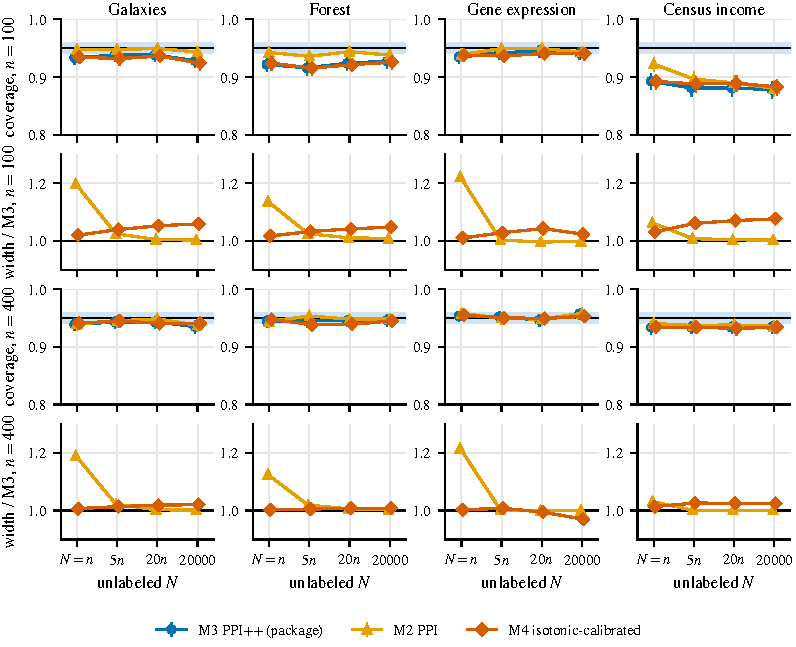
\includegraphics[width=\linewidth]{../figures/real_nsweep.pdf}
\caption{Dependence on the unlabeled sample size $N\in\{n,5n,20n,20000\}$ at $n=100$ and $400$.}
\label{fig:nsweep}
\end{figure}

\begin{figure}[h]
\centering
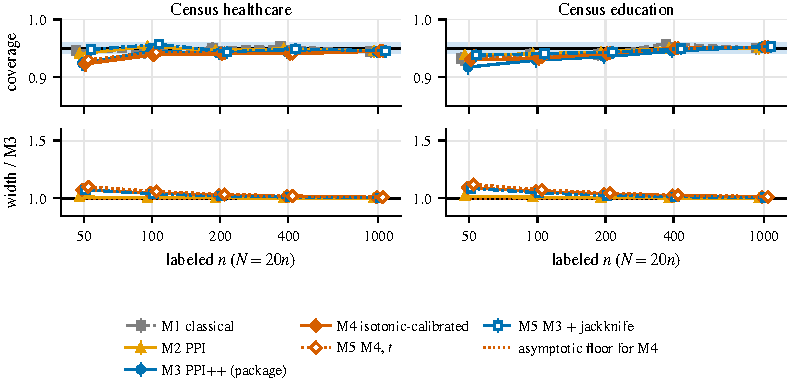
\includegraphics[width=\linewidth]{../figures/real_appendix.pdf}
\caption{Census healthcare and education, $N=20n$.}
\label{fig:realapp}
\end{figure}


\begin{table}[h]
\caption{Bootstrap ablation ($R=1000$): unclipped PPI++ (\texttt{ppipp\_nc}) against percentile and studentized bootstrap.}
\label{tab:boot}
\centering\scriptsize
\adjustbox{max width=\linewidth}{\begin{tabular}{lrrrrrrr}
\toprule
Dataset & $n$ & $N$ & PPI++ cov. & boot. pct cov. & boot. pct width / PPI++ & boot. $t$ cov. & boot. $t$ width / PPI++ \\
\midrule
AlphaFold & 50 & 250 & \textbf{0.907} & \textbf{0.912} & 1.141 & 0.943 & 1.201 \\
AlphaFold & 50 & 1000 & \textbf{0.880} & \textbf{0.871} & 1.209 & \textbf{0.914} & 1.235 \\
AlphaFold & 100 & 500 & \textbf{0.934} & \textbf{0.928} & 1.075 & 0.962 & 1.103 \\
AlphaFold & 100 & 2000 & \textbf{0.915} & \textbf{0.915} & 1.118 & 0.959 & 1.127 \\
AlphaFold & 200 & 1000 & 0.943 & 0.946 & 1.036 & 0.950 & 1.053 \\
AlphaFold & 200 & 4000 & 0.945 & 0.947 & 1.064 & 0.956 & 1.070 \\
Ballots & 50 & 250 & \textbf{0.934} & \textbf{0.936} & 1.095 & 0.958 & 1.105 \\
Ballots & 50 & 1000 & \textbf{0.935} & 0.953 & 1.208 & 0.946 & 1.194 \\
Ballots & 100 & 500 & 0.945 & 0.948 & 1.041 & 0.956 & 1.045 \\
Ballots & 100 & 2000 & 0.937 & 0.941 & 1.084 & \textbf{0.931} & 1.106 \\
Ballots & 200 & 1000 & 0.956 & 0.951 & 1.014 & 0.956 & 1.017 \\
Ballots & 200 & 4000 & 0.952 & 0.950 & 1.036 & 0.944 & 1.052 \\
Census income & 50 & 250 & \textbf{0.838} & \textbf{0.844} & 1.002 & \textbf{0.903} & 1.427 \\
Census income & 50 & 1000 & \textbf{0.810} & \textbf{0.819} & 1.046 & \textbf{0.885} & 1.487 \\
Census income & 100 & 500 & \textbf{0.878} & \textbf{0.880} & 0.999 & \textbf{0.913} & 1.269 \\
Census income & 100 & 2000 & \textbf{0.867} & \textbf{0.866} & 1.009 & \textbf{0.896} & 1.295 \\
Census income & 200 & 1000 & \textbf{0.916} & \textbf{0.914} & 0.991 & \textbf{0.931} & 1.139 \\
Census income & 200 & 4000 & \textbf{0.902} & \textbf{0.907} & 0.999 & \textbf{0.931} & 1.160 \\
Forest & 50 & 250 & \textbf{0.910} & \textbf{0.908} & 1.068 & \textbf{0.927} & 1.180 \\
Forest & 50 & 1000 & \textbf{0.926} & \textbf{0.919} & 1.106 & 0.942 & 1.184 \\
Forest & 100 & 500 & \textbf{0.922} & \textbf{0.924} & 1.032 & 0.966 & 1.094 \\
Forest & 100 & 2000 & \textbf{0.912} & \textbf{0.920} & 1.052 & 0.962 & 1.103 \\
Forest & 200 & 1000 & 0.949 & 0.946 & 1.013 & 0.956 & 1.043 \\
Forest & 200 & 4000 & \textbf{0.933} & \textbf{0.933} & 1.023 & 0.952 & 1.048 \\
Galaxies & 50 & 250 & \textbf{0.926} & \textbf{0.927} & 1.057 & 0.951 & 1.121 \\
Galaxies & 50 & 1000 & \textbf{0.909} & \textbf{0.905} & 1.069 & 0.949 & 1.125 \\
Galaxies & 100 & 500 & 0.949 & 0.944 & 1.026 & 0.961 & 1.054 \\
Galaxies & 100 & 2000 & \textbf{0.930} & \textbf{0.930} & 1.037 & 0.943 & 1.061 \\
Galaxies & 200 & 1000 & 0.937 & \textbf{0.936} & 1.006 & 0.938 & 1.018 \\
Galaxies & 200 & 4000 & 0.943 & 0.943 & 1.014 & 0.946 & 1.026 \\
Gene expression & 50 & 250 & \textbf{0.931} & 0.941 & 1.095 & 0.959 & 1.092 \\
Gene expression & 50 & 1000 & \textbf{0.931} & 0.949 & 1.175 & 0.959 & 1.120 \\
Gene expression & 100 & 500 & 0.957 & 0.964 & 1.044 & 0.962 & 1.043 \\
Gene expression & 100 & 2000 & 0.938 & 0.947 & 1.085 & 0.955 & 1.059 \\
Gene expression & 200 & 1000 & 0.938 & 0.939 & 1.020 & 0.948 & 1.020 \\
Gene expression & 200 & 4000 & 0.947 & 0.944 & 1.047 & 0.956 & 1.033 \\
\bottomrule
\end{tabular}
}
\end{table}

\begin{table}[h]
\caption{Forest, labeled draws with versus without replacement.}
\label{tab:wor}
\centering\scriptsize
\adjustbox{max width=\linewidth}{\begin{tabular}{rrrrrrr}
\toprule
$n$ & M3 cov., with repl. & M4 cov., with repl. & M4 / M3, with repl. & M3 cov., without repl. & M4 cov., without repl. & M4 / M3, without repl. \\
\midrule
50 & \textbf{0.923} & \textbf{0.923} & 1.076 & \textbf{0.908} & \textbf{0.906} & 1.079 \\
100 & \textbf{0.924} & \textbf{0.921} & 1.041 & \textbf{0.936} & \textbf{0.930} & 1.043 \\
200 & \textbf{0.929} & \textbf{0.933} & 1.022 & 0.952 & 0.949 & 1.025 \\
\bottomrule
\end{tabular}
}
\end{table}

\begin{table}[h]
\caption{Intervals on one realisation at native dataset sizes (10\% labeled, 90\% unlabeled, seed 0); descriptive only, no coverage claim.}
\label{tab:native}
\centering\scriptsize
\adjustbox{max width=\linewidth}{\begin{tabular}{lrrllrl}
\toprule
Dataset & n & N & Method & Interval & Width & Covers $\theta$ \\
\midrule
Galaxies & 1674 & 15069 & M1 classical & [0.2447, 0.2870] & 0.04234 & True \\
Galaxies & 1674 & 15069 & M2 PPI & [0.2518, 0.2823] & 0.03045 & True \\
Galaxies & 1674 & 15069 & ppipp & [0.2518, 0.2820] & 0.03020 & True \\
Galaxies & 1674 & 15069 & M4 isotonic-calibrated & [0.2509, 0.2813] & 0.03041 & True \\
Galaxies & 1674 & 15069 & binned-calibrated & [0.2517, 0.2823] & 0.03058 & True \\
Galaxies & 1674 & 15069 & spline-calibrated & [0.2518, 0.2821] & 0.03031 & True \\
Forest & 159 & 1437 & M1 classical & [0.1387, 0.2638] & 0.1250 & True \\
Forest & 159 & 1437 & M2 PPI & [0.1411, 0.2525] & 0.1114 & True \\
Forest & 159 & 1437 & ppipp & [0.1422, 0.2528] & 0.1106 & True \\
Forest & 159 & 1437 & M4 isotonic-calibrated & [0.1364, 0.2516] & 0.1152 & True \\
Forest & 159 & 1437 & binned-calibrated & [0.1319, 0.2510] & 0.1191 & True \\
Forest & 159 & 1437 & spline-calibrated & [0.1357, 0.2518] & 0.1161 & True \\
AlphaFold & 1080 & 9722 & M1 classical & [0.1585, 0.2045] & 0.04599 & True \\
AlphaFold & 1080 & 9722 & M2 PPI & [0.1711, 0.2011] & 0.03000 & True \\
AlphaFold & 1080 & 9722 & ppipp & [0.1708, 0.2007] & 0.02988 & True \\
AlphaFold & 1080 & 9722 & M4 isotonic-calibrated & [0.1699, 0.2001] & 0.03021 & True \\
AlphaFold & 1080 & 9722 & binned-calibrated & [0.1686, 0.1995] & 0.03088 & True \\
AlphaFold & 1080 & 9722 & spline-calibrated & [0.1703, 0.2004] & 0.03010 & True \\
Gene expression & 6115 & 55035 & M1 classical & [6.637, 6.859] & 0.2217 & True \\
Gene expression & 6115 & 55035 & M2 PPI & [6.738, 6.829] & 0.09035 & True \\
Gene expression & 6115 & 55035 & ppipp & [6.738, 6.829] & 0.09035 & True \\
Gene expression & 6115 & 55035 & M4 isotonic-calibrated & [6.742, 6.832] & 0.08982 & True \\
Gene expression & 6115 & 55035 & binned-calibrated & [6.746, 6.838] & 0.09231 & True \\
Gene expression & 6115 & 55035 & spline-calibrated & [6.742, 6.832] & 0.08962 & True \\
Census income & 38009 & 342082 & M1 classical & [42062, 43574] & 1512 & True \\
Census income & 38009 & 342082 & M2 PPI & [42278, 43520] & 1242 & True \\
Census income & 38009 & 342082 & ppipp & [42278, 43520] & 1242 & True \\
Census income & 38009 & 342082 & M4 isotonic-calibrated & [42230, 43458] & 1228 & True \\
Census income & 38009 & 342082 & binned-calibrated & [42400, 43659] & 1259 & True \\
Census income & 38009 & 342082 & spline-calibrated & [42225, 43453] & 1229 & True \\
Census healthcare & 31821 & 286394 & M1 classical & [0.6634, 0.6738] & 0.01034 & True \\
Census healthcare & 31821 & 286394 & M2 PPI & [0.6651, 0.6728] & 0.007706 & True \\
Census healthcare & 31821 & 286394 & ppipp & [0.6651, 0.6728] & 0.007659 & True \\
Census healthcare & 31821 & 286394 & M4 isotonic-calibrated & [0.6652, 0.6729] & 0.007656 & True \\
Census healthcare & 31821 & 286394 & binned-calibrated & [0.6651, 0.6728] & 0.007684 & True \\
Census healthcare & 31821 & 286394 & spline-calibrated & [0.6652, 0.6728] & 0.007657 & True \\
Census education & 31821 & 286394 & M1 classical & [17.76, 17.86] & 0.09654 & True \\
Census education & 31821 & 286394 & M2 PPI & [17.78, 17.85] & 0.07835 & True \\
Census education & 31821 & 286394 & ppipp & [17.78, 17.85] & 0.07790 & True \\
Census education & 31821 & 286394 & M4 isotonic-calibrated & [17.78, 17.85] & 0.07797 & True \\
Census education & 31821 & 286394 & binned-calibrated & [17.78, 17.86] & 0.07850 & True \\
Census education & 31821 & 286394 & spline-calibrated & [17.78, 17.85] & 0.07790 & True \\
Ballots & 1027 & 78150 & M1 classical & [0.5985, 0.6576] & 0.05915 & NaN \\
Ballots & 1027 & 78150 & M2 PPI & [0.6145, 0.6278] & 0.01330 & NaN \\
Ballots & 1027 & 78150 & ppipp & [0.6149, 0.6280] & 0.01313 & NaN \\
Ballots & 1027 & 78150 & M4 isotonic-calibrated & [0.6149, 0.6281] & 0.01320 & NaN \\
Ballots & 1027 & 78150 & binned-calibrated & [0.6149, 0.6281] & 0.01320 & NaN \\
Ballots & 1027 & 78150 & spline-calibrated & [0.6149, 0.6281] & 0.01320 & NaN \\
Plankton & 421238 & 329832 & M1 classical & [0.1327, 0.1348] & 0.002056 & False \\
Plankton & 421238 & 329832 & M2 PPI & [0.06890, 0.07097] & 0.002069 & False \\
Plankton & 421238 & 329832 & ppipp & [0.1038, 0.1054] & 0.001582 & False \\
Plankton & 421238 & 329832 & M4 isotonic-calibrated & [0.1038, 0.1054] & 0.001582 & False \\
Plankton & 421238 & 329832 & binned-calibrated & [0.1038, 0.1054] & 0.001582 & False \\
Plankton & 421238 & 329832 & spline-calibrated & [0.1038, 0.1054] & 0.001582 & False \\
\bottomrule
\end{tabular}
}
\end{table}

\begin{figure}[h]
\centering
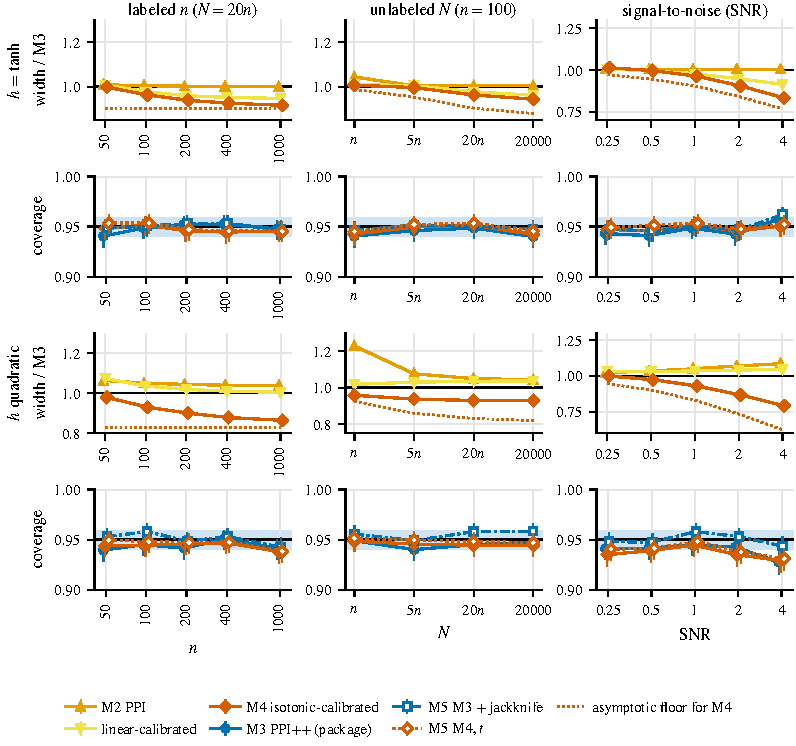
\includegraphics[width=\linewidth]{../figures/synthetic_factors.pdf}
\caption{Synthetic populations: width ratio to M3 and coverage versus $n$, $N$ and SNR ($\kappa=0.5$).}
\label{fig:synfac}
\end{figure}

\begin{table}[h]
\caption{Heavy-tailed (Student-$t_3$) noise: coverage and paired width ratio of M4 to M3 (95\% bootstrap interval).}
\label{tab:tail}
\centering\scriptsize
\adjustbox{max width=\linewidth}{\begin{tabular}{lllrrrl}
\toprule
$h$ & $\kappa$ & tail & M3 cov. & M4 cov. & M5 (M3) cov. & M4 / M3 \\
\midrule
quad & 0.0 & Student-$t_3$ & 0.950 & 0.952 & 0.958 & 1.061 [1.060, 1.063] \\
quad & 0.5 & Student-$t_3$ & 0.945 & 0.942 & 0.951 & 0.919 [0.916, 0.922] \\
tanh & 0.0 & Student-$t_3$ & 0.947 & 0.948 & 0.955 & 1.061 [1.060, 1.063] \\
tanh & 0.5 & Student-$t_3$ & 0.951 & 0.953 & 0.956 & 0.952 [0.950, 0.954] \\
\bottomrule
\end{tabular}
}
\end{table}

The spline calibrator (not the frozen M4) on the quadratic family, $n=100$, $N=20n$: paired width ratio to M3 $1.086$, $0.996$, $0.933$, $0.882$, $0.827$ for $\kappa=0,0.25,0.5,0.75,1$ against ceilings $1.000$, $0.903$, $0.830$, $0.773$, $0.726$ (\texttt{code/results/theory\_check\_synth\_final.csv}); isotonic gives $1.060$, $0.979$, $0.930$, $0.912$, $0.948$.

\begin{table}[h]
\caption{Coverage at $n=100$ and $400$, $R=2000$; bold: Wilson upper bound below $0.95$. All cells: \texttt{figures/tables/tab\_real\_full.csv}.}
\label{tab:cov}
\centering\scriptsize
\adjustbox{max width=\linewidth}{\begin{tabular}{lrrrrrrrr}
\toprule
Dataset & $n$ & $R$ & M3 & M1 & M2 & M4 & M5 (M3) & M5 (M4) \\
\midrule
Galaxies & 100 & 2000 & \textbf{0.939} & 0.945 & 0.950 & \textbf{0.936} & 0.956 & \textbf{0.940} \\
Galaxies & 400 & 2000 & 0.944 & \textbf{0.940} & 0.949 & 0.941 & 0.949 & 0.942 \\
Forest & 100 & 2000 & \textbf{0.924} & \textbf{0.932} & 0.944 & \textbf{0.921} & \textbf{0.940} & \textbf{0.924} \\
AlphaFold & 100 & 2000 & \textbf{0.922} & \textbf{0.930} & 0.945 & \textbf{0.902} & 0.948 & \textbf{0.904} \\
AlphaFold & 400 & 2000 & \textbf{0.939} & 0.951 & 0.942 & \textbf{0.940} & 0.945 & \textbf{0.940} \\
Gene expression & 100 & 2000 & 0.945 & 0.950 & 0.950 & 0.941 & 0.959 & 0.945 \\
Gene expression & 400 & 2000 & 0.947 & 0.948 & 0.948 & 0.949 & 0.951 & 0.951 \\
Census income & 100 & 2000 & \textbf{0.881} & \textbf{0.909} & \textbf{0.890} & \textbf{0.889} & \textbf{0.898} & \textbf{0.891} \\
Census income & 400 & 2000 & \textbf{0.934} & \textbf{0.936} & \textbf{0.938} & \textbf{0.932} & 0.942 & \textbf{0.933} \\
Ballots & 100 & 2000 & \textbf{0.934} & 0.942 & \textbf{0.940} & \textbf{0.935} & 0.946 & \textbf{0.938} \\
\bottomrule
\end{tabular}
}
\end{table}

\begin{table}[h]
\caption{Mean width of M3 and paired width ratios to M3 ($\pm$ half the 95\% bootstrap interval).}
\label{tab:realwidth}
\centering\scriptsize
\adjustbox{max width=\linewidth}{\begin{tabular}{lrrrrrrr}
\toprule
Dataset & $n$ & M3 mean width & M1 / M3 & M2 / M3 & M4 / M3 & M5 (M3) / M3 & M5 (M4) / M3 \\
\midrule
Galaxies & 100 & 0.118 & 1.457 $\pm$ 0.007 & 1.005 $\pm$ 0.001 & 1.052 $\pm$ 0.002 & 1.051 $\pm$ 0.002 & 1.065 $\pm$ 0.002 \\
Galaxies & 400 & 0.0592 & 1.450 $\pm$ 0.003 & 1.003 $\pm$ 0.000 & 1.019 $\pm$ 0.001 & 1.015 $\pm$ 0.001 & 1.022 $\pm$ 0.001 \\
Forest & 100 & 0.119 & 1.185 $\pm$ 0.004 & 1.010 $\pm$ 0.001 & 1.041 $\pm$ 0.002 & 1.057 $\pm$ 0.003 & 1.054 $\pm$ 0.002 \\
AlphaFold & 100 & 0.0897 & 1.673 $\pm$ 0.012 & 0.996 $\pm$ 0.001 & 1.073 $\pm$ 0.004 & 1.084 $\pm$ 0.005 & 1.087 $\pm$ 0.004 \\
AlphaFold & 400 & 0.0453 & 1.653 $\pm$ 0.005 & 0.999 $\pm$ 0.000 & 1.023 $\pm$ 0.001 & 1.026 $\pm$ 0.001 & 1.027 $\pm$ 0.001 \\
Gene expression & 100 & 0.605 & 2.849 $\pm$ 0.012 & 0.996 $\pm$ 0.001 & 1.042 $\pm$ 0.002 & 1.046 $\pm$ 0.003 & 1.055 $\pm$ 0.002 \\
Gene expression & 400 & 0.302 & 2.852 $\pm$ 0.006 & 1.000 $\pm$ 0.000 & 0.995 $\pm$ 0.001 & 1.007 $\pm$ 0.001 & 0.998 $\pm$ 0.001 \\
Census income & 100 & 22836 & 1.273 $\pm$ 0.005 & 1.004 $\pm$ 0.000 & 1.070 $\pm$ 0.004 & 1.049 $\pm$ 0.003 & 1.083 $\pm$ 0.004 \\
Census income & 400 & 11966 & 1.236 $\pm$ 0.002 & 1.001 $\pm$ 0.000 & 1.025 $\pm$ 0.002 & 1.010 $\pm$ 0.001 & 1.028 $\pm$ 0.002 \\
Ballots & 100 & 0.0539 & 3.592 $\pm$ 0.033 & 1.020 $\pm$ 0.001 & 1.012 $\pm$ 0.001 & 1.063 $\pm$ 0.006 & 1.024 $\pm$ 0.000 \\
\bottomrule
\end{tabular}
}
\end{table}
